% PA3 report skeleton. Structure, figure/table slots and data wiring only.
% All prose (abstract, methods, analysis, captions) must be written by the author:
% the PA3 policy forbids generative-AI-written report text. Fill every [AUTHOR] marker.
\documentclass{article}
\usepackage[preprint]{neurips_2026}
\usepackage[utf8]{inputenc}
\usepackage[T1]{fontenc}
\usepackage{amsmath,amssymb,graphicx,booktabs,caption,microtype,array}
\usepackage[hidelinks]{hyperref}
\setcitestyle{authoryear,square,comma}
\graphicspath{{figures/}}
\newcommand{\AUTHOR}[1]{\textcolor{red}{[AUTHOR: #1]}}
\usepackage{xcolor}

\title{\AUTHOR{title}}
\author{\AUTHOR{name, roll number}}

\begin{document}
\maketitle

\begin{abstract}
\AUTHOR{abstract}. Code: \url{[LINK REQUIRED: public GitHub repository]}
\end{abstract}

\section{Introduction}
\AUTHOR{brief introduction}

\section{Experimental setup}
\AUTHOR{concise methods for Tasks 1--3; deviations from the prescribed setup (see README, ``Implementation choices'')}

% =====================================================================
\section{Task 1: LLM fine-tuning}
\subsection{Results and analysis}
% RQ1 specialization/retention, RQ2 restrictions, RQ3 parameter changes, RQ4 cost, RQ5 behavior

\begin{table}[t]
\centering\small
\begin{tabular}{lcccc}
\toprule
Condition & GSM8K & HellaSwag & BoolQ & ARC-Easy \\
\midrule
Baseline & 43.14 & 47.32 & 64.37 & 56.06 \\
Full FT (mid) & 57.01 (+13.87) & 45.69 (-1.63) & 59.94 (-4.43) & 62.04 (+5.98) \\
Full FT & 64.44 (+21.30) & 45.89 (-1.43) & 58.90 (-5.47) & 63.59 (+7.53) \\
Full FT + L2-SP & 64.90 (+21.76) & 46.53 (-0.79) & 67.52 (+3.15) & 63.43 (+7.37) \\
LoRA-4 & 60.12 (+16.98) & 47.40 (+0.08) & 69.69 (+5.32) & 63.51 (+7.45) \\
LoRA-16 & 62.02 (+18.88) & 47.03 (-0.29) & 70.83 (+6.45) & 63.43 (+7.37) \\
OPLoRA-16 & 61.33 (+18.20) & 47.16 (-0.16) & 70.06 (+5.69) & 63.09 (+7.03) \\
\bottomrule
\end{tabular}
\caption{\AUTHOR{caption: benchmark scores for the seven evaluation conditions, changes from baseline in pp}}
\label{tab:t1-bench}
\end{table}

\begin{figure}[t]
\centering
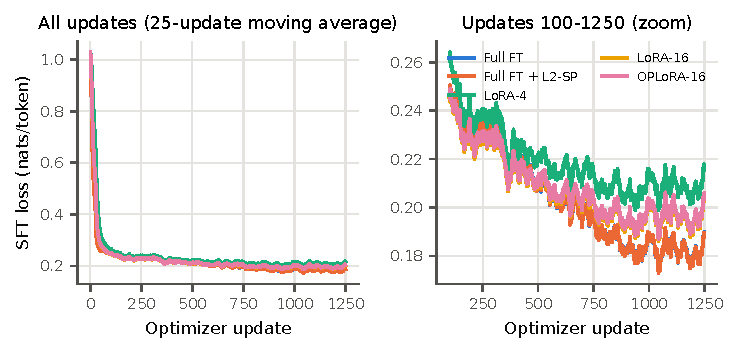
\includegraphics[width=0.55\linewidth]{task1/sft_loss.pdf}\hfill
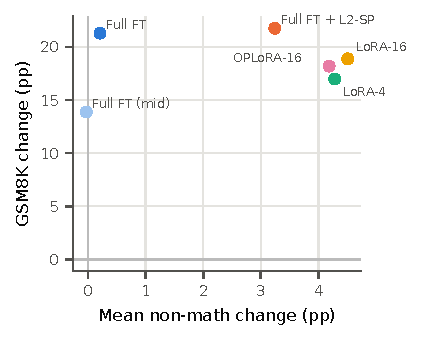
\includegraphics[width=0.42\linewidth]{task1/tradeoff.pdf}
\caption{\AUTHOR{caption: SFT loss curves; GSM8K change vs mean non-math change}}
\label{fig:t1-loss}
\end{figure}

\begin{table}[t]
\centering\small
\begin{tabular}{lrrrr}
\toprule
Method & Trainable params & Train time (h) & Peak mem. (GB) & Final ckpt (MB) \\
\midrule
Full FT & 596,049,920 & 2.47 & 11.12 & 2395.7 \\
Full FT + L2-SP & 596,049,920 & 2.58 & 12.23 & 2395.7 \\
LoRA-4 & 2,523,136 & 2.85 & 2.26 & 20.4 \\
LoRA-16 & 10,092,544 & 2.80 & 2.37 & 80.9 \\
OPLoRA-16 & 10,092,544 & 3.74 & 2.68 & 80.9 \\
\bottomrule
\end{tabular}
\caption{\AUTHOR{caption: resources}}
\label{tab:t1-res}
\end{table}

\begin{figure}[t]
\centering
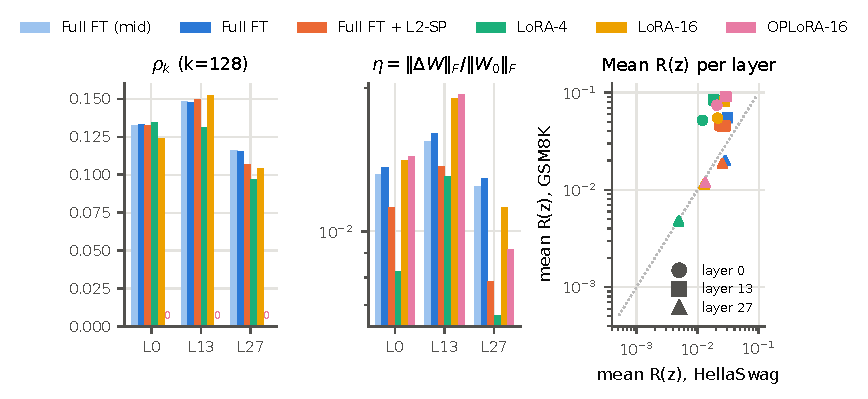
\includegraphics[width=\linewidth]{task1/diagnostics.pdf}
\caption{\AUTHOR{caption: $\rho_k$, $\eta$ and $R(z)$ on down\_proj, layers 0/13/27}}
\label{fig:t1-diag}
\end{figure}

\AUTHOR{analysis organised by the five research questions; L2-SP penalty and displacement
(results/task1/train/*/summary.json, figures/task1/l2sp\_penalty.pdf); qualitative findings
from results/task1/qualitative/annotation\_sheet\_42.csv}

% =====================================================================
\section{Task 2: Vision-language model and visual grounding}
\subsection{Results and analysis}
% RQ1 visual interface, RQ2 grounding, RQ3 measuring image use, RQ4 capabilities and cost

\begin{figure}[t]
\centering
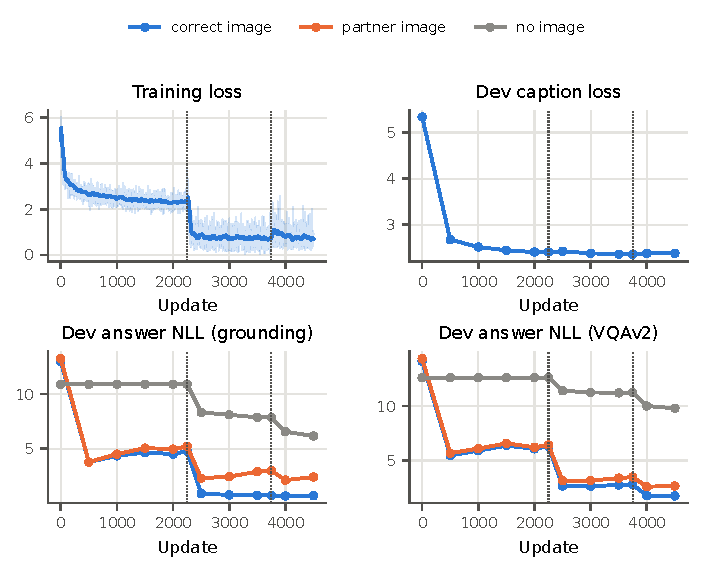
\includegraphics[width=\linewidth]{task2/learning_curves.pdf}
\caption{\AUTHOR{caption: training loss, dev caption loss and answer NLL by image condition; dotted lines mark stage boundaries}}
\label{fig:t2-curves}
\end{figure}

\begin{table}[t]
\centering\small
\resizebox{\linewidth}{!}{\begin{tabular}{llcccccc}
\toprule
Suite & Image & Acc. & Pair acc. & Identical & Empty & Ref. NLL & s/answer \\
\midrule
Grounding & correct & 64.1 [54.7, 73.4] & 50.0 & 17.2 & 0.0 & 0.818 & 0.036 \\
Grounding & complementary & 12.5 [7.0, 18.0] & 1.6 & 17.2 & 0.0 & 2.692 & 0.032 \\
Grounding & mismatched & 43.0 [36.7, 49.2] & 6.2 & 67.2 & 0.0 & 1.603 & 0.033 \\
Grounding & none & 0.0 [0.0, 0.0] & 0.0 & 100.0 & 0.0 & 6.426 & 0.110 \\
\midrule
VQAv2 & correct & 54.1 [46.8, 61.3] & 27.1 & 49.0 & 0.0 & 1.330 & 0.039 \\
VQAv2 & complementary & 27.9 [22.5, 33.4] & 1.0 & 49.0 & 0.0 & 2.160 & 0.039 \\
VQAv2 & mismatched & 35.0 [28.7, 41.7] & 6.2 & 60.4 & 0.0 & 1.996 & 0.037 \\
VQAv2 & none & 0.0 [0.0, 0.0] & 0.0 & 100.0 & 0.0 & 9.021 & 0.123 \\
\bottomrule
\end{tabular}}
\caption{\AUTHOR{caption: final-test results under four image conditions, 95\% pair-bootstrap intervals}}
\label{tab:t2-final}
\end{table}

\AUTHOR{analysis; qualitative examples from results/task2/eval/qualitative\_examples.json with the stated selection rule; resources from results/task2/summary/resources.json}

% =====================================================================
\section{Task 3: Test-time compute}
\subsection{Results and analysis}
% RQ1 exploration/selection, RQ2 evidence/consensus, RQ3 breadth/refinement, RQ4 adaptive, RQ5 compute/reliability

\begin{figure}[t]
\centering
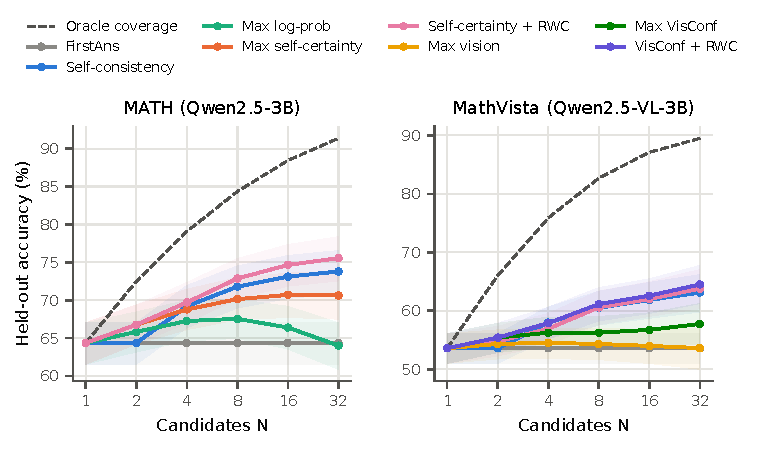
\includegraphics[width=\linewidth]{task3/accuracy_vs_n.pdf}
\caption{\AUTHOR{caption: held-out accuracy and oracle coverage vs candidate budget}}
\label{fig:t3-acc}
\end{figure}

\begin{figure}[t]
\centering
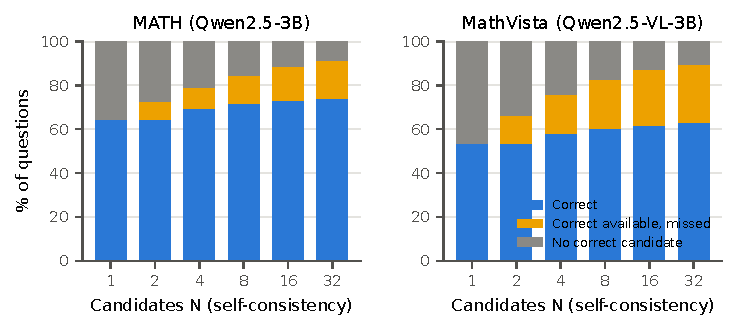
\includegraphics[width=\linewidth]{task3/failure_decomposition.pdf}
\caption{\AUTHOR{caption: sampling vs selection failures}}
\label{fig:t3-dec}
\end{figure}

\begin{table}[t]
\centering\small
\begin{tabular}{lcc}
\toprule
Method & MATH & MathVista \\
\midrule
FirstAns & 64.3 [61.5, 67.0] & 53.6 [51.0, 56.1] \\
Self-consistency & 73.8 [70.8, 76.6] & 63.1 [59.8, 66.2] \\
Max log-prob & 64.0 [60.9, 67.0] & 48.1 [44.6, 51.5] \\
Max self-certainty & 70.6 [67.5, 73.8] & 54.6 [51.1, 58.1] \\
Self-certainty + RWC & 75.5 [72.5, 78.4] & 63.8 [60.4, 67.0] \\
Log-prob + RWC & 74.9 [72.0, 77.8] & 61.4 [58.0, 64.5] \\
Shortest & 62.4 [59.0, 65.5] & 53.8 [50.5, 56.9] \\
Max vision & -- & 53.6 [50.0, 57.0] \\
Vision + RWC & -- & 63.9 [60.5, 67.1] \\
Max VisConf & -- & 57.8 [54.2, 61.3] \\
VisConf + RWC & -- & 64.5 [61.2, 67.8] \\
Max tokenwise VisConf & -- & 56.2 [52.8, 59.4] \\
Tokenwise VisConf + RWC & -- & 63.9 [60.5, 67.1] \\
\bottomrule
\end{tabular}
\caption{\AUTHOR{caption: method comparison at $N=32$, held-out split}}
\label{tab:t3-methods}
\end{table}

\AUTHOR{signal analysis (results/task3/signals/), live comparison (results/task3/summary/live.csv,
results/task3/live/meta.json), adaptive stopping (results/task3/summary/adaptive.csv)}

\section{Conclusion}
\AUTHOR{brief conclusion}

\bibliographystyle{plainnat}
\bibliography{references}

\appendix
\section{Additional results}
\AUTHOR{appendix}
\end{document}
